\newpage\section{Evaluation of the solution}

To validate the developed prototype, the previously established test cases are verified for the individual requirements. The testing of the test cases provides information about the degree of fulfillment of the requirements. In addition, the fulfillment of requirements that could not be validated by test cases is considered. Subsequently, the usability of the \ac{ui} of the prototype is assessed.

\subsection{Prototype validation}
This section looks at the individual test cases from Section \ref{subsec:requirement_validation} and describes both their implementation and the degree to which they have been fulfilled. Furthermore, the fulfillment of requirements that cannot be confirmed by test cases is evaluated. 

\newpage\subsubsection*{T1: A welcome and goodbye message is displayed} 

The implementation of this test case can be done without further development by utilizing the standard functionalities of the developed prototype. For this purpose, the Information Screen Activity is specified as the first and last step in the experiment data. Furthermore, a corresponding welcome and farewell text is stored in the experiment data. Figure \ref{fig:T1} shows that the functional requirements F1.1 and F2.1 to show information at the beginning of the experiment and to provide the participants with debrifing information can be completely fulfilled by the artefact.

\vspace{1.5cm}

\begin{figure}[htbp]
    \centering
    \begin{subfigure}[b]{0.25\textwidth}
        \centering
        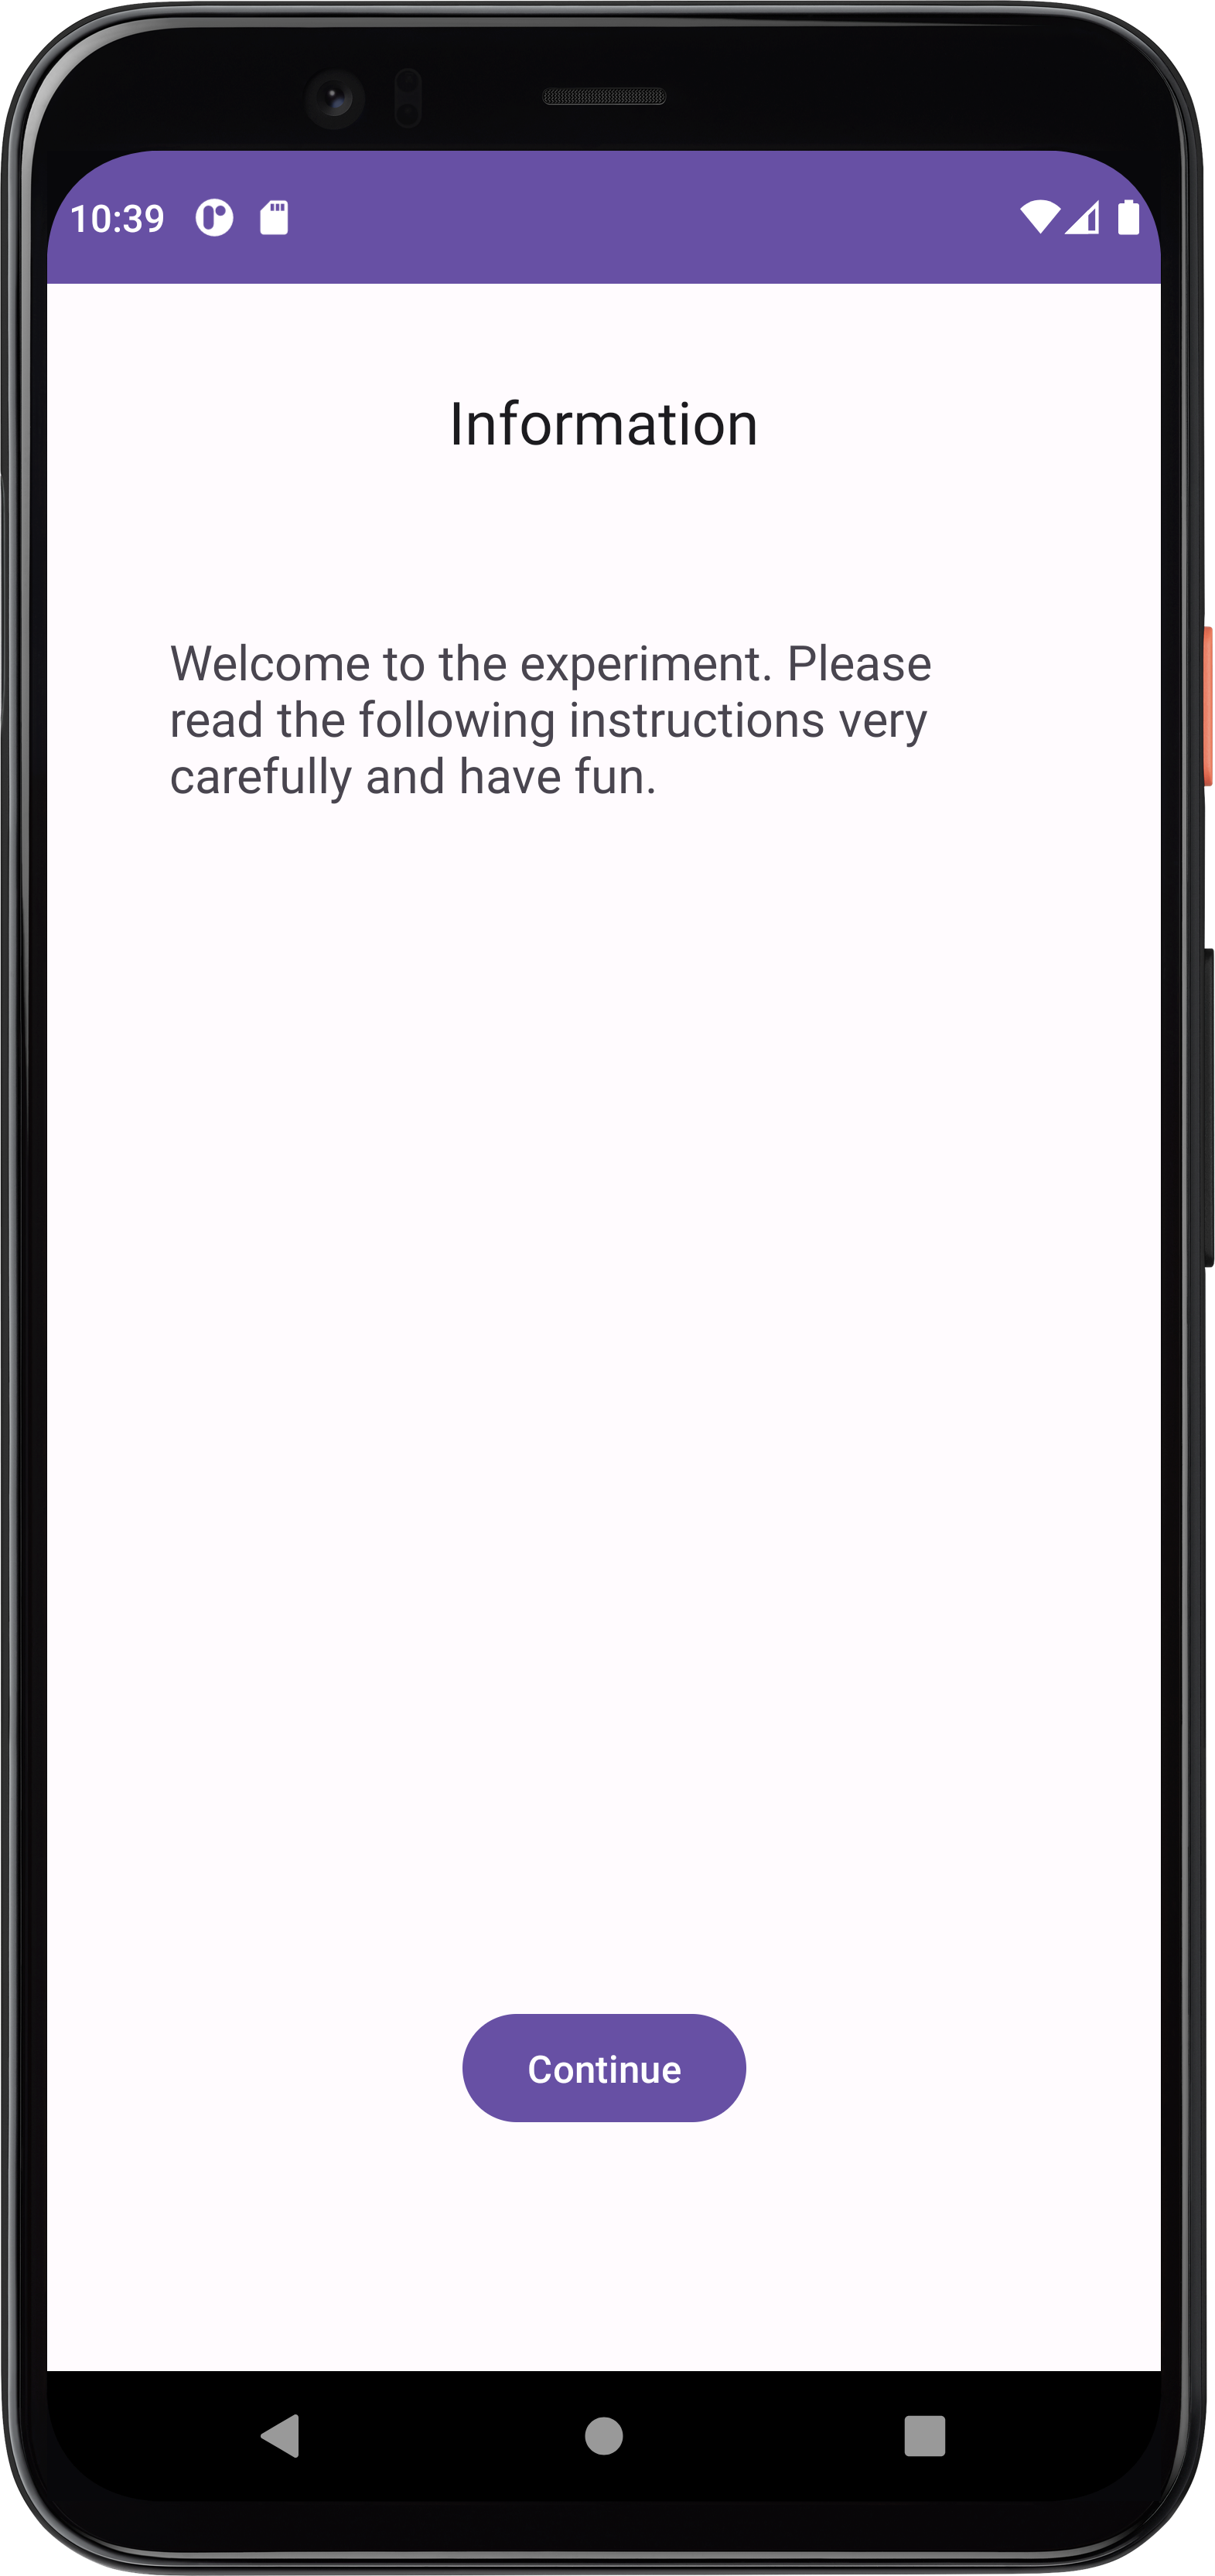
\includegraphics[width=\textwidth]{content/07_evaluation_of_the_solution/Screenshot_StartingScreen.png}
        \caption{Welcome Message}
        \label{subfig:welcomeMessage}
    \end{subfigure}
    \hspace{1cm}
    \begin{subfigure}[b]{0.25\textwidth}
        \centering
        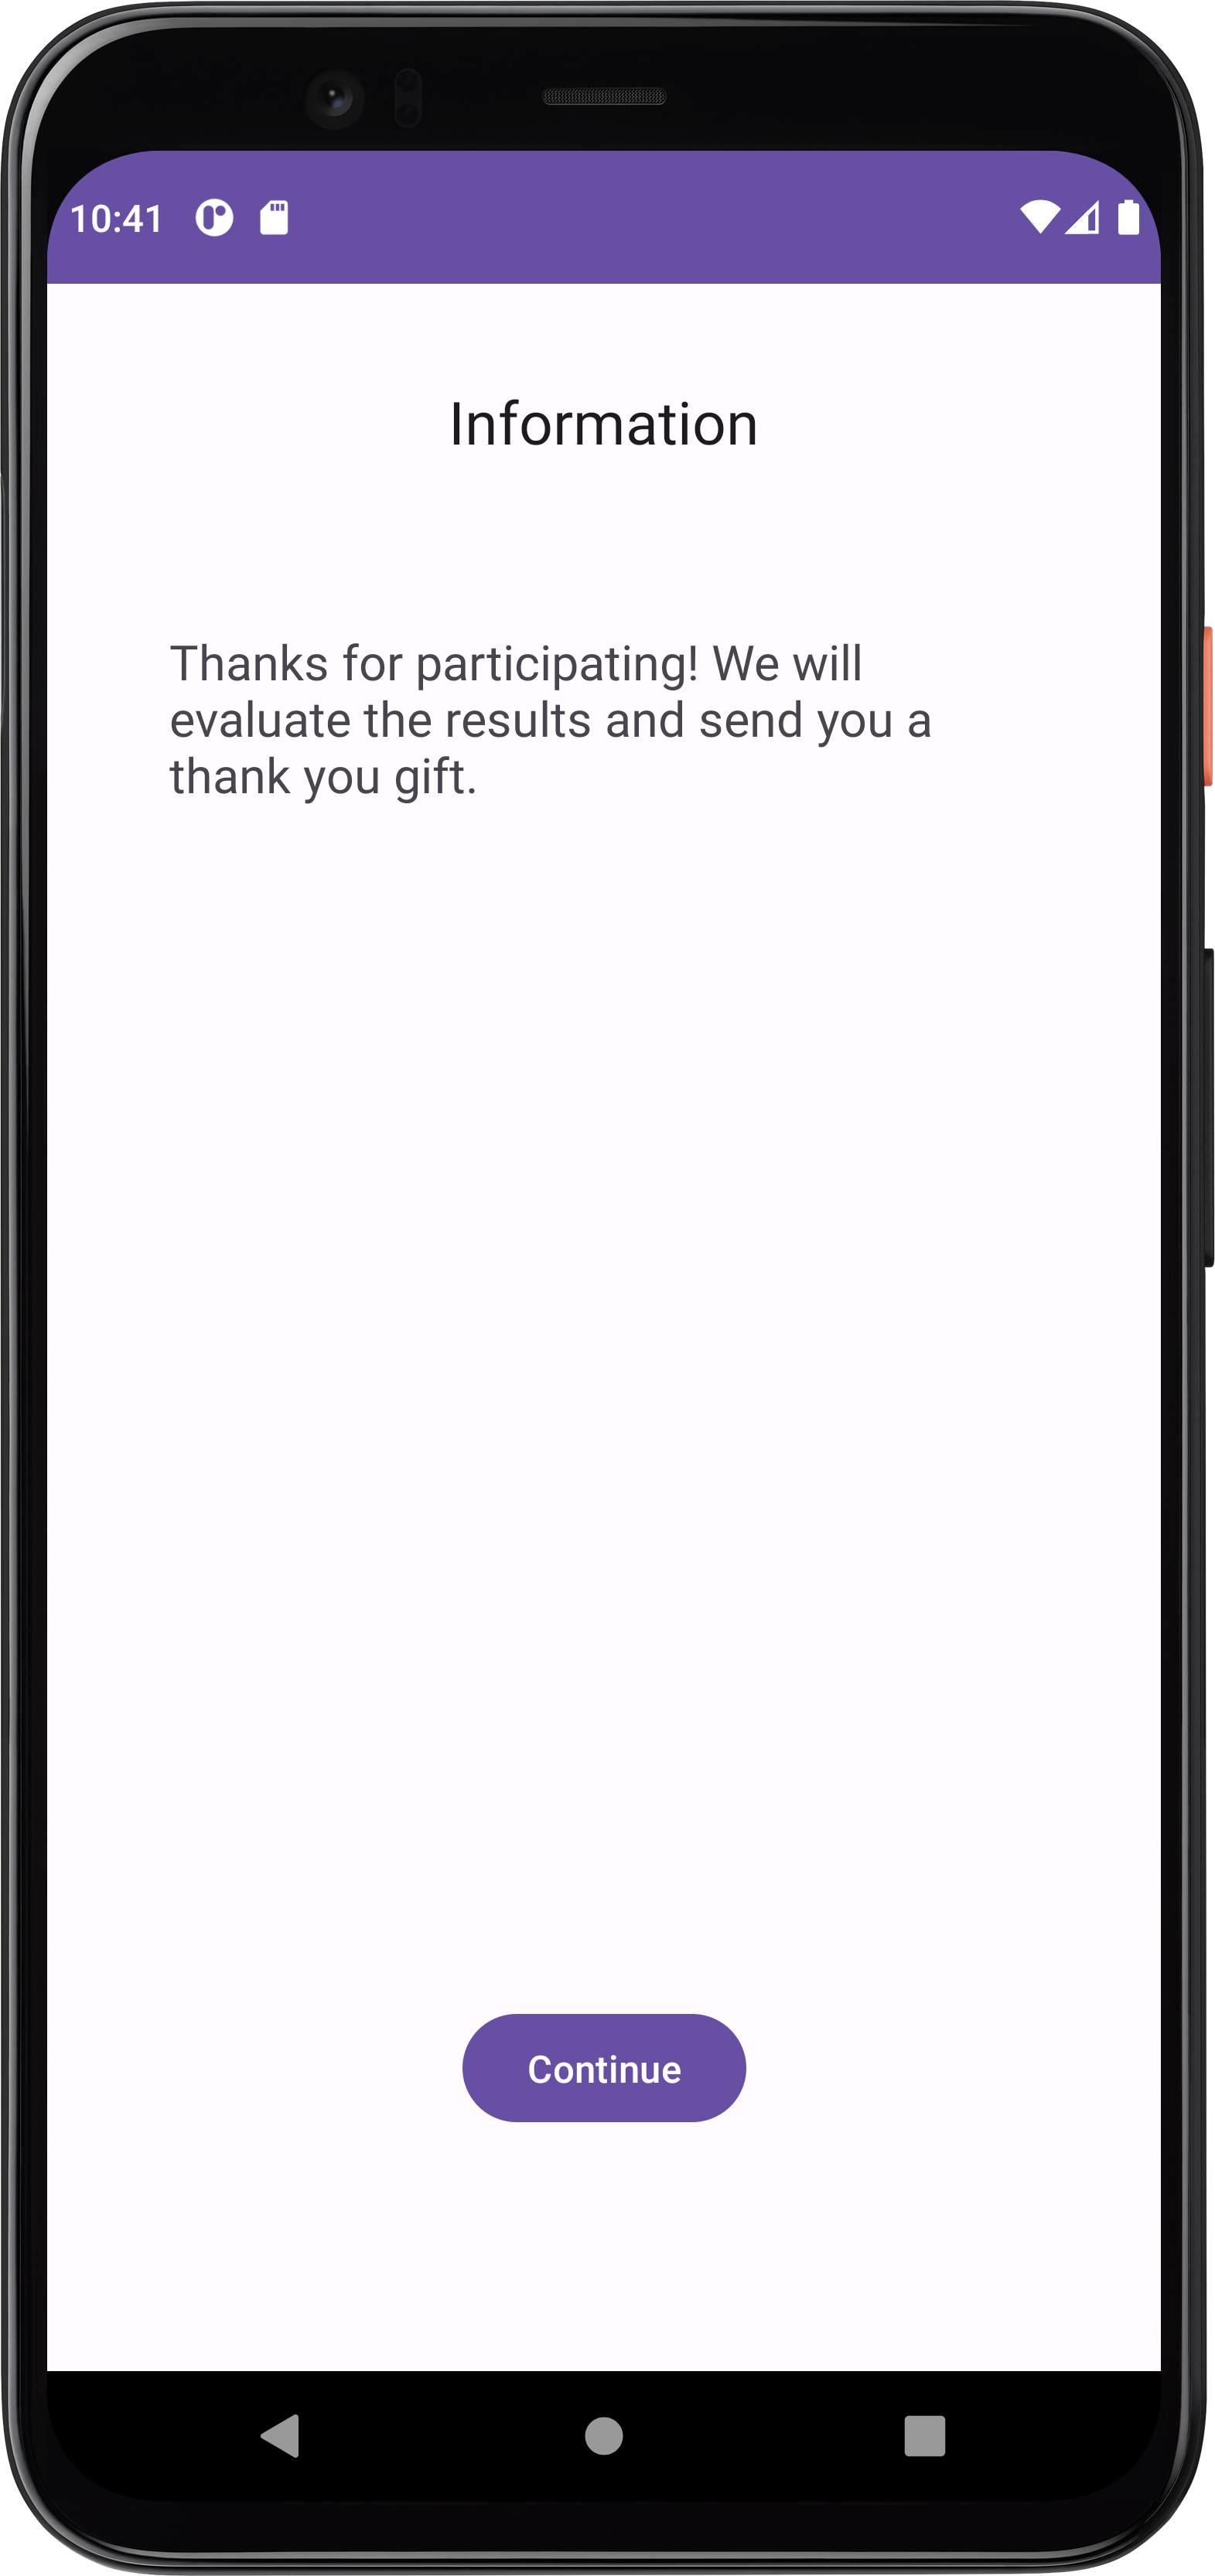
\includegraphics[width=\textwidth]{content/07_evaluation_of_the_solution/Screenshot_GoodbyeMessage.png}
        \caption{Goodbye Message}
        \label{subfig:goodbyeMessage}
    \end{subfigure}
    \caption{User Interface Testcase T1}
    \label{fig:T1}
\end{figure}

\newpage\subsubsection*{T2: Participants are prompted to input their age at the beginning and prompted to input how the liked the experiment at the end}

To perform this test, the experiment data must also be adjusted first. For this, the questionnair step must be placed at the beginning and the end of the experiment step order within the experiment data. In addition, the participant data must contain the respective data as an empty field to be queried as an attribute, since the query of the questionnair process only queries for missing data. These data entries are \enquote{age} and \enquote{experiment feedback} as defined by the test case. The two screens on which the participants are asked for their age at the beginning of the experiment and for feedback on the experiment at its end are shown in Figure \ref{fig:T2}. The test T2 and thus the requirements F2.1, F2.3, F2.2 and F2.3 can thus be fulfilled.

\vspace{0.5cm}

\begin{figure}[htbp]
    \centering
    \begin{subfigure}[b]{0.25\textwidth}
        \centering
        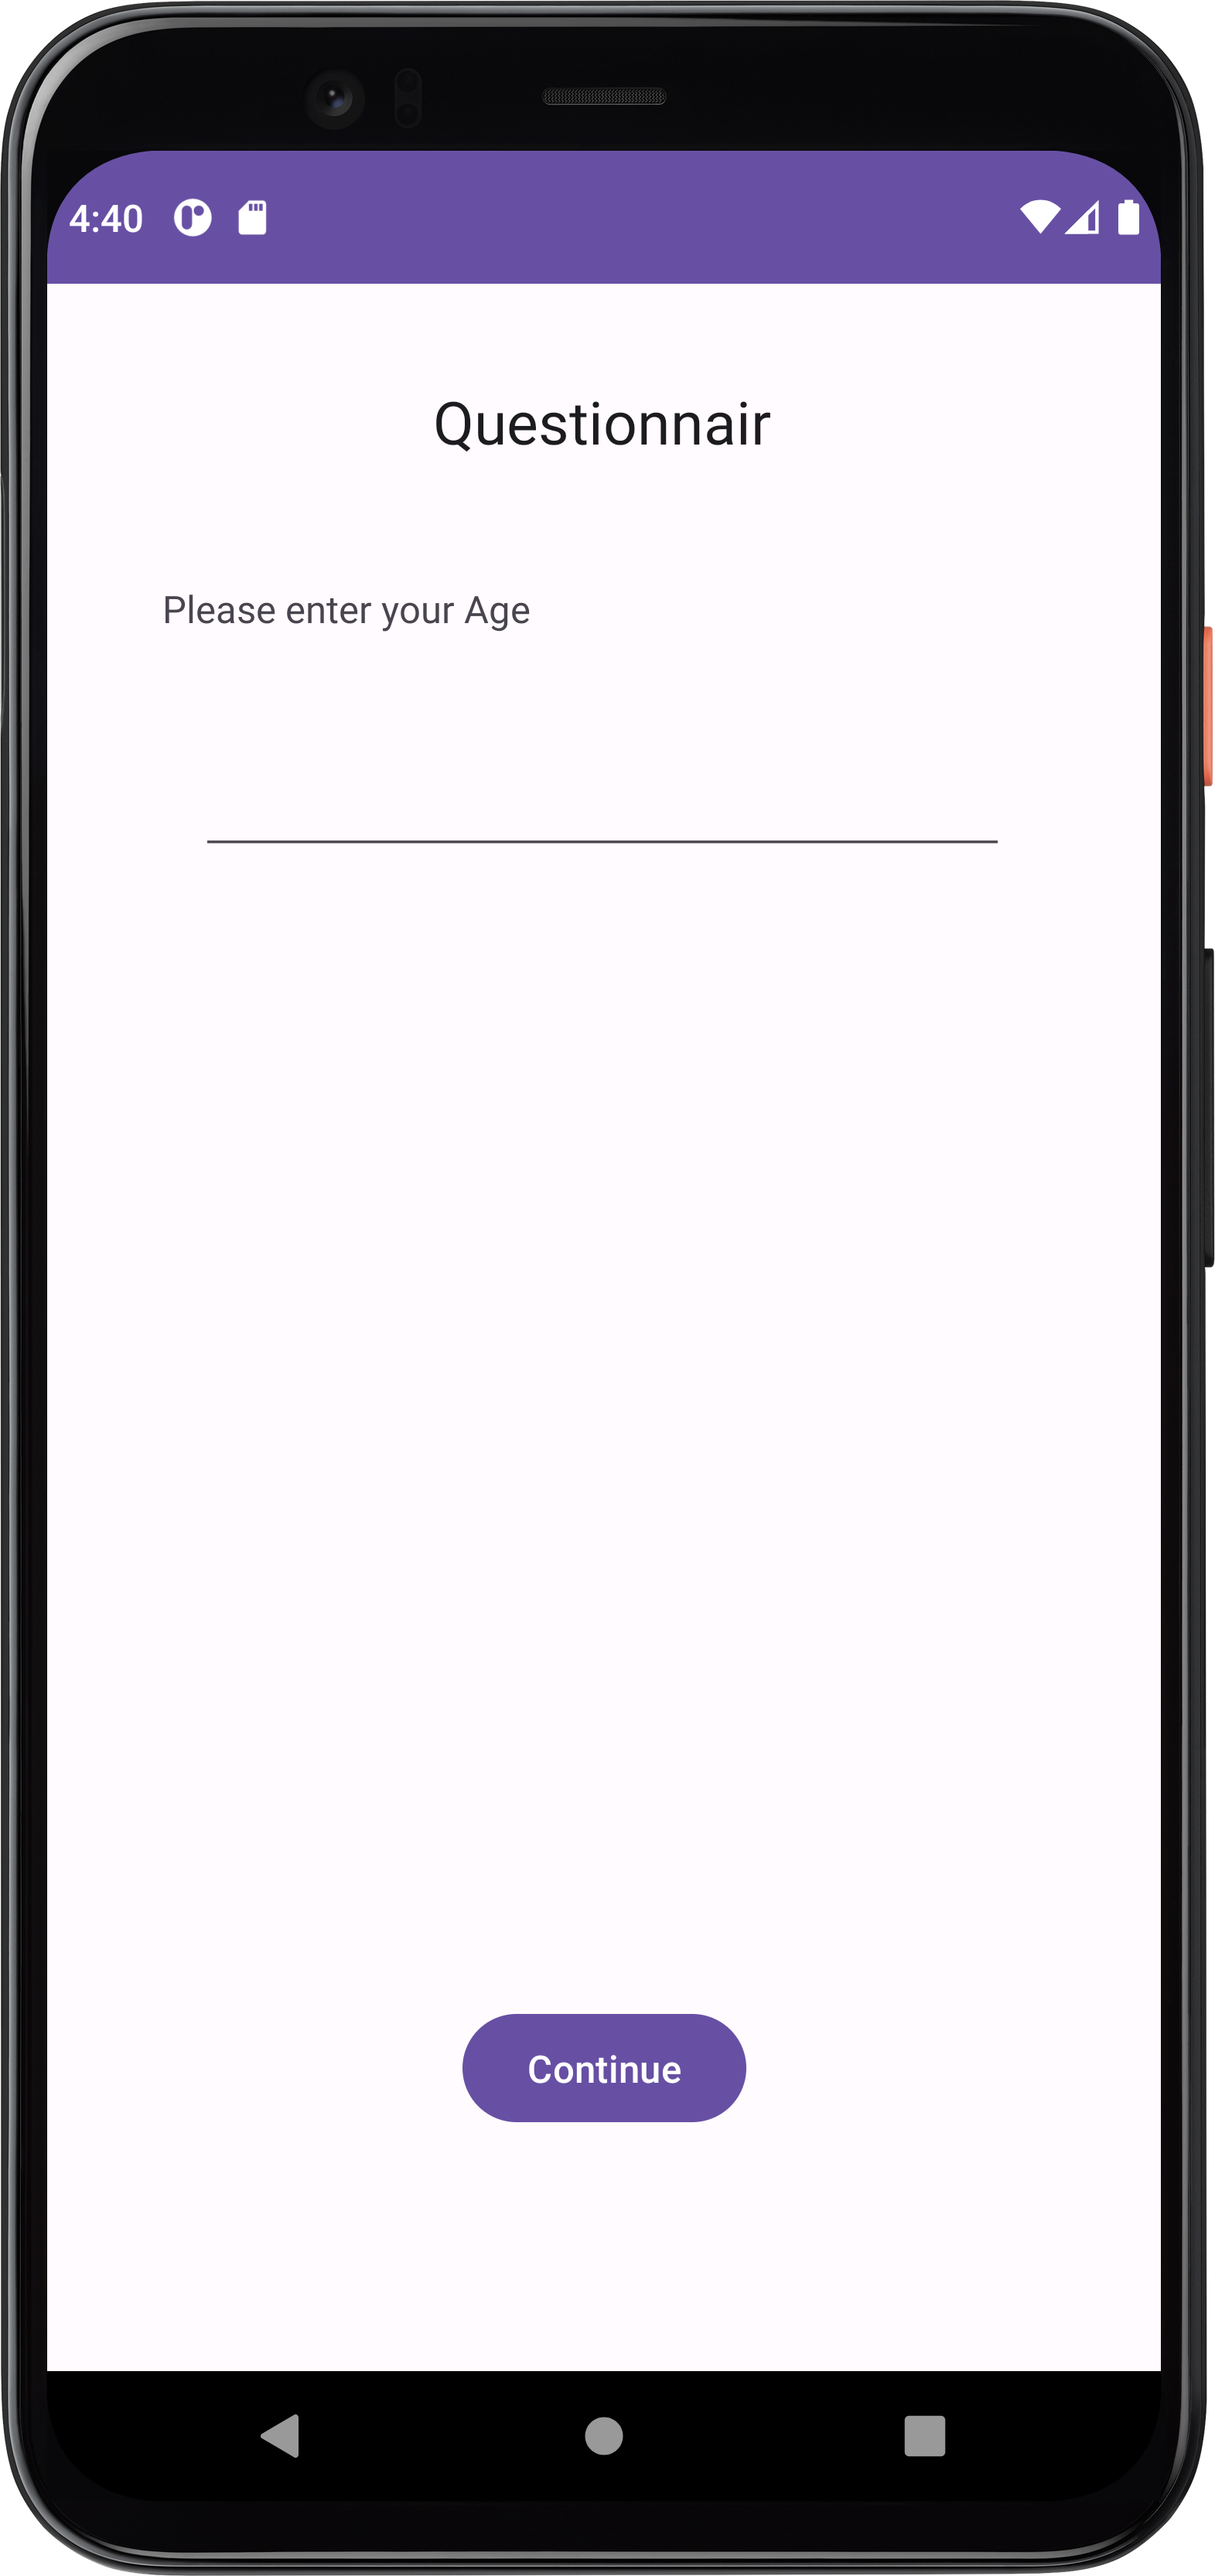
\includegraphics[width=\textwidth]{content/07_evaluation_of_the_solution/Screenshot_T2a.png}
        \caption{Welcome Message}
        \label{subfig:t2a}
    \end{subfigure}
    \hspace{1cm}
    \begin{subfigure}[b]{0.25\textwidth}
        \centering
        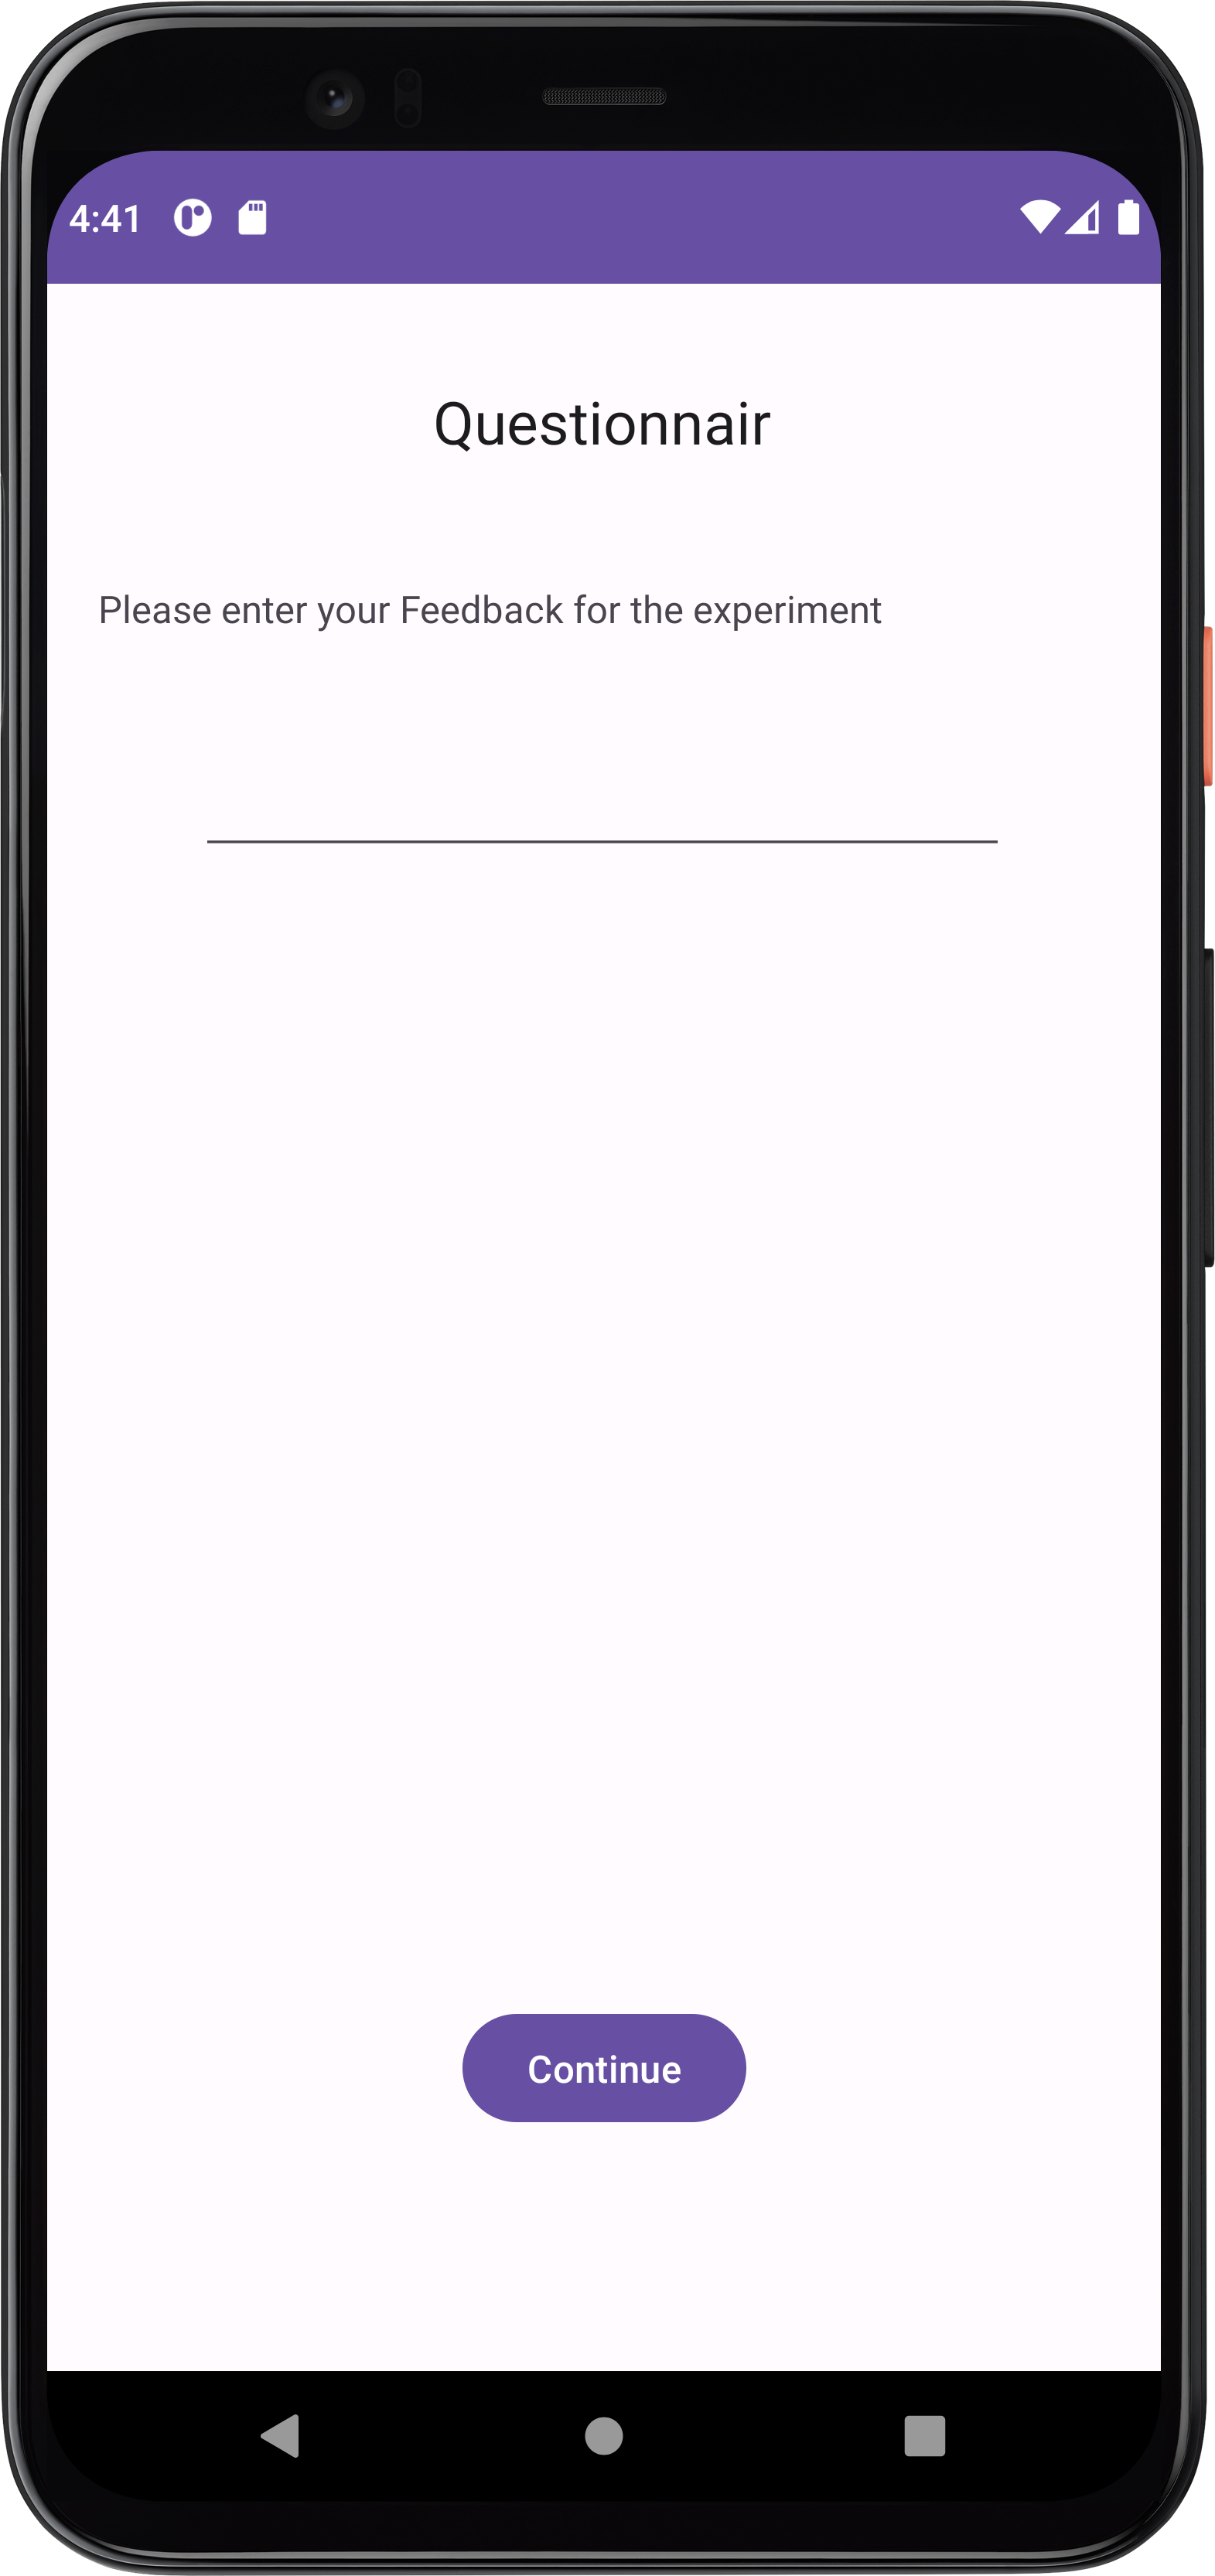
\includegraphics[width=\textwidth]{content/07_evaluation_of_the_solution/Screenshot_T2b.png}
        \caption{Goodbye Message}
        \label{subfig:t2b}
    \end{subfigure}
    \caption{User Interface Testcase T1}
    \label{fig:T2}
\end{figure}

\newpage\subsubsection*{T3: The information about how long the experiment took is collected}

To fulfill this test case, which checks requirement F2.2, the time necessary to perform the experiment is measured. For this, the lines of code from Listing \ref{t3a} can be used on the start activity. These store the start time of the experiment in the meta data in the experiment data. The experiment is then run and the code lines in Listing \ref{t3b} are called when the experiment is completed. These code lines retrieve the start time of the experiment from the experiment data and calculate the total elapsed time during the experiment using the current system time. This is then also stored in the meta data of the experiment data. Thus, the test case T3 can be completely fulfilled and consequently the requirement F2.2.

\vspace{1cm}

\begin{lstlisting}[language=java,label=t3a,lineskip={0pt}, caption=Collect time needed to conduct experiment (a), basicstyle=\scriptsize, captionpos=b]
    String currentTime = new SimpleDateFormat("HH:mm:ss", Locale.getDefault()).format(new Date());
    LogMetaDataUseCase.getInstance().setMetaData(currentTime);
\end{lstlisting}

\begin{lstlisting}[language=java,label=t3b,lineskip={0pt}, caption=Collect time needed to conduct experiment (b), basicstyle=\scriptsize, captionpos=b]
    long difference = date1.getTime() - date2.getTime();
    LogMetaDataUseCase.getInstance().setMetaData(difference);
\end{lstlisting}


\newpage\subsubsection*{T4: The gender and the weight of the participant is pre-loaded into the experiment from different files. The gender of the participant is deleted}

For test case T4, which verifies requirement F3.2, the files to be read in are read via corresponding Java interfaces in the ParticipantData class. Java supports the import of a variety of different file formats (\cite{Ullenboom.2017}). At the same time, the read-in data can also be formatted or adapted. In test case T4, the gender and weight of the participants is read in and the information about the gender is then deleted.

\vspace{1cm}

\begin{lstlisting}[language=java,label=t3b,lineskip={0pt}, caption=Collect time needed to conduct experiment (b), basicstyle=\scriptsize, captionpos=b]
    File csvfile = new File(Environment.getExternalStorageDirectory() + "/participantData.csv");
    CSVReader reader = new CSVReader(new FileReader(csvfile.getAbsolutePath()));
    String[] nextLine;
    while ((nextLine = reader.readNext()) != null) {
        // nextLine[] is an array of values from the line
        ParticipantEntity participant = new ParticipantEntity(Integer.parseInt(nextLine[0]));
        participant.setName(nextLine[0]);
        participant.setEducation(nextLine[0]);
        participant.setGender(null);
    
        data.add(participant);
    }
\end{lstlisting}

\newpage\subsubsection*{T5: A chess game is added as custom logic}

In test case T5, a chessboard game is to be implemented following the study of X. This test case is intended to verify F2.1, F2.2 and F2.3 which deal with the implementation of custom logic. The chessboard serves as a proof of the functionality to implement custom logic in the application. Since the checkerboard is an experimental step that requires interaction with the user, this test case is implemented in the course of a new activity. This activity has to be added to the order of the activities in the experiment data to ensure that it is called. A screenshot of this activity is shown in figure \ref{fig:chess}. The detailed coding of this custom activity will not be discussed further, since it only serves to verify the requirements. Through this custom activity and the fact that Java is a Turing Complete programming language testcase T5 is fulfilled.

\vspace{1.5cm}

\begin{figure}[htbp]
    \centering
    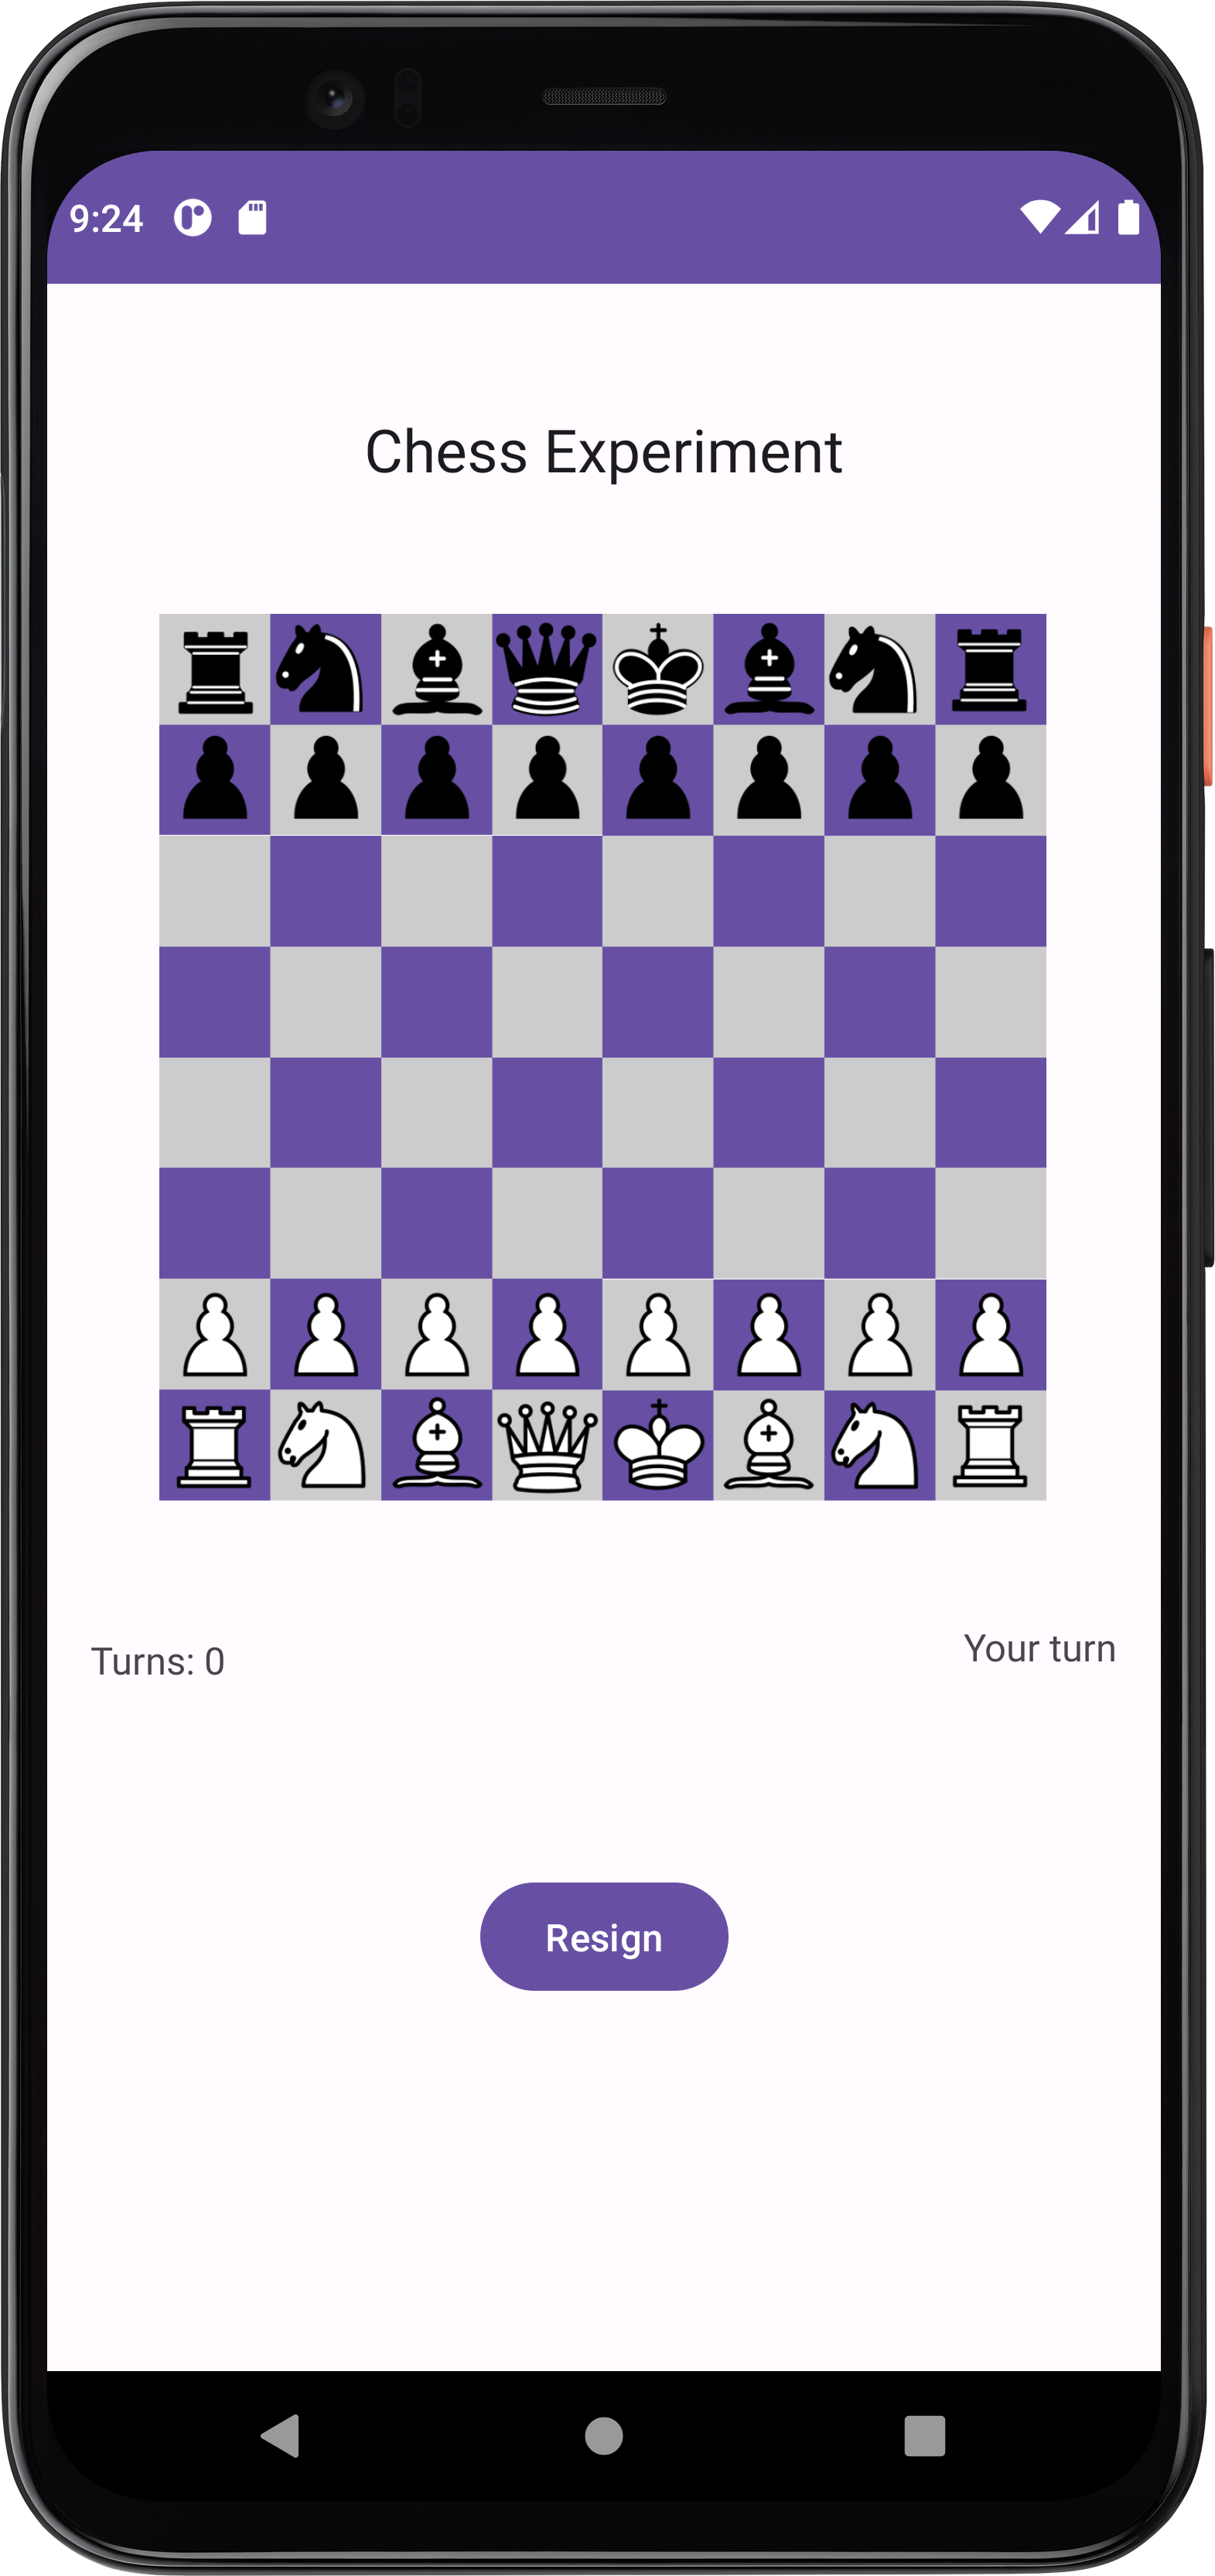
\includegraphics[width=0.3\textwidth, keepaspectratio]{content/07_evaluation_of_the_solution/Screenshot_Chess.png}
    \caption{Custom experiment logic}    
    \label{fig:chess}
\end{figure}

\newpage\subsubsection*{T6: Two groups are created, one of the groups is particularly chosen the other one randomly selected}

%the first one through putting the group into the respective participant data
%second through code within the use case:
Generally, groups are defined by adding a group ID (e.g. group A or group 1) in the user data. If the corresponding group assignment field is not filled, the assignment is performed automatically in the AllocateGroupsUseCase use case. The code snippet in Listing \ref{t6} shows the standard code that assigns the participants who have no group assignment to a random group. The corresponding group assignment is then stored in the previously empty attribute. The test case T6 and thus the requirements F4.1, F4.3 and F4.4 are verified. Furthermore, a customized or extended group assignment would be implemented in the AllocateGroupsUseCase use case.

\vspace{1cm}

\begin{lstlisting}[language=java,label=t6,lineskip={0pt}, caption=Collect time needed to conduct experiment (b), basicstyle=\scriptsize, captionpos=b]
    currentParticipant = getCurrentParticipantUseCase.getCurrentParticipant();
    currentParticipantGroup = participantRepository.getParticipant(currentParticipant).getGroupAllocation();
    
    if(currentParticipantGroup == null){
    
        if(experimentRepository.getExperiment().getGroupAllocation() == "random"){
            Random random = new Random();
            int randomNumber = random.nextInt(2); // Generates either 0 or 1
    
            if(randomNumber == 0 ){
                setGroupAllocationPUseCase.setGroupAllocation("Group A", currentParticipant);
            } else {
                setGroupAllocationPUseCase.setGroupAllocation("Group B", currentParticipant);
            }
        };
    }
\end{lstlisting}

\newpage\subsubsection*{T7: A chess turn is played by both parties not using the same device}

Test case T7 deals with the interaction between multiple participants. For this purpose, the chess game in test case T5 is to be played by several participants on different devices. The implementation of this test case lies in the corresponding activity itself. In this case in the ChessGameActivity. For this a client class is needed for sending the current game state and a server class for receiving and offering the current game state. These classes are nested as private classes in the activity itself. Listing A shows the code for the server class, Listing B the code for the client class and Listing C the initiation of both classes at the start of the chess game. The server and client are initiated using threads to ensure correct and fast communication between the two playing parties. In this way, after each move played, the current state of the board is sent via the client of one device to the server of the other device. Since this test case only serves as a proof-of-concept, Java sockets were used to implement the communication. These are characterized by their simplicity, but their functionality is limited, especially for modern applications. The use of third-party interfaces or externally hosted servers such as Firebase is therefore conceivable, depending on the requirements of the experiment (\cite{Google.2023b}). Communication between two experiment participants on different devices could be demonstrated by playing a chess move in each case. Test case T7 and thus requirements F4.2, N1.1 and N1.2 could thus be fulfilled and confirmed.

\vspace{1cm}

\begin{lstlisting}[language=java,label=t7b,lineskip={0pt}, caption=Collect time needed to conduct experiment (b), basicstyle=\scriptsize, captionpos=b]
    private class ClientThread extends Thread {
        @Override
        public void run() {
            try {
                Socket socket = new Socket(server_ip, server_port);
                PrintWriter out = new PrintWriter(socket.getOutputStream(), true);
                out.println(message);
                out.close();
                socket.close();
            } catch (IOException e) {
                e.printStackTrace();
            }
        }
    }
\end{lstlisting}

\begin{lstlisting}[language=java,label=t7a,lineskip={0pt}, caption=Collect time needed to conduct experiment (b), basicstyle=\scriptsize, captionpos=b]
private class ServerThread extends Thread {
        @Override
        public void run() {
            try {
                ServerSocket serverSocket = new ServerSocket(client_port);
                Socket clientSocket = serverSocket.accept();

                BufferedReader in = new BufferedReader(new InputStreamReader(clientSocket.getInputStream()));
                String message = in.readLine();
                in.close();
                clientSocket.close();
                serverSocket.close();

                handleMessage(message);

            } catch (IOException e) {
                e.printStackTrace();
            }
        }
    }
\end{lstlisting}

\begin{lstlisting}[language=java,label=t7c,lineskip={0pt}, caption=Collect time needed to conduct experiment (b), basicstyle=\scriptsize, captionpos=b]
    new ClientThread().start();
    new ServerThread().start();
\end{lstlisting}

\newpage\subsubsection*{T8 :The results of the experiment are retrieved and displayed in third party software}

To fulfill test case T8 and thus verify requirements N3.1, N.3.2, meta data are exported from the application and then read into external software. As mentioned above, Android in combination with Java basically supports a variety of file formats for export. The export of the metadata is implemented in the LogMetaDataUseCase use case via the printOutMetaData method and is shown in Listing \ref{t8}. For simplicity and as a proof of concept in the course of this test case, meta data in the form of processing times for the experiment is exported as a CSV file. These are then read into Excel in the course of this test case and visualized using an Excel representation. Figure \ref{fig:Excel} shows this Excel graphic. In principle, however, the CSV file could be processed in any other way, provided that the software used for further processing supports CSV files. 

\vspace{1cm}


\begin{lstlisting}[language=java,label=t8,lineskip={0pt}, caption=Collect time needed to conduct experiment (b), basicstyle=\scriptsize, captionpos=b]
    File file = new File(Environment.getExternalStorageDirectory() + "/participant" + GetCurrentParticipantUseCase.getInstance().getCurrentParticipant() + "TimeData.csv");
    try {
        // create FileWriter object with file as parameter
        FileWriter outputfile = new FileWriter(file);

        // create CSVWriter object filewriter object as parameter
        CSVWriter writer = new CSVWriter(outputfile);

        // adding header to csv
        String[] header = { "id", "time in milliseconds"};
        writer.writeNext(header);

        //Getting participant information
        ArrayList<ParticipantEntity> participantEntities = GetParticipantDataUseCase.getInstance().getParticipantData();

        //Writing current participant time into file
        //String[] data = {String.valueOf(GetCurrentParticipantUseCase.getInstance().getCurrentParticipant()), String.valueOf(timeDifference)};

        Iterator iter = participantEntities.iterator();
        while (iter.hasNext()) {
            String[] data = {String.valueOf(((ParticipantEntity)iter.next()).getId()), String.valueOf(((ParticipantEntity)iter.next()).getExperimentTime())};
            writer.writeNext(data);
        }
        //closing writer connection
        writer.close();
    }
    catch (IOException e) {
        // TODO Auto-generated catch block
        e.printStackTrace();
        System.out.println("Error");
    }
\end{lstlisting}

\begin{figure}[htbp]
    \centering
    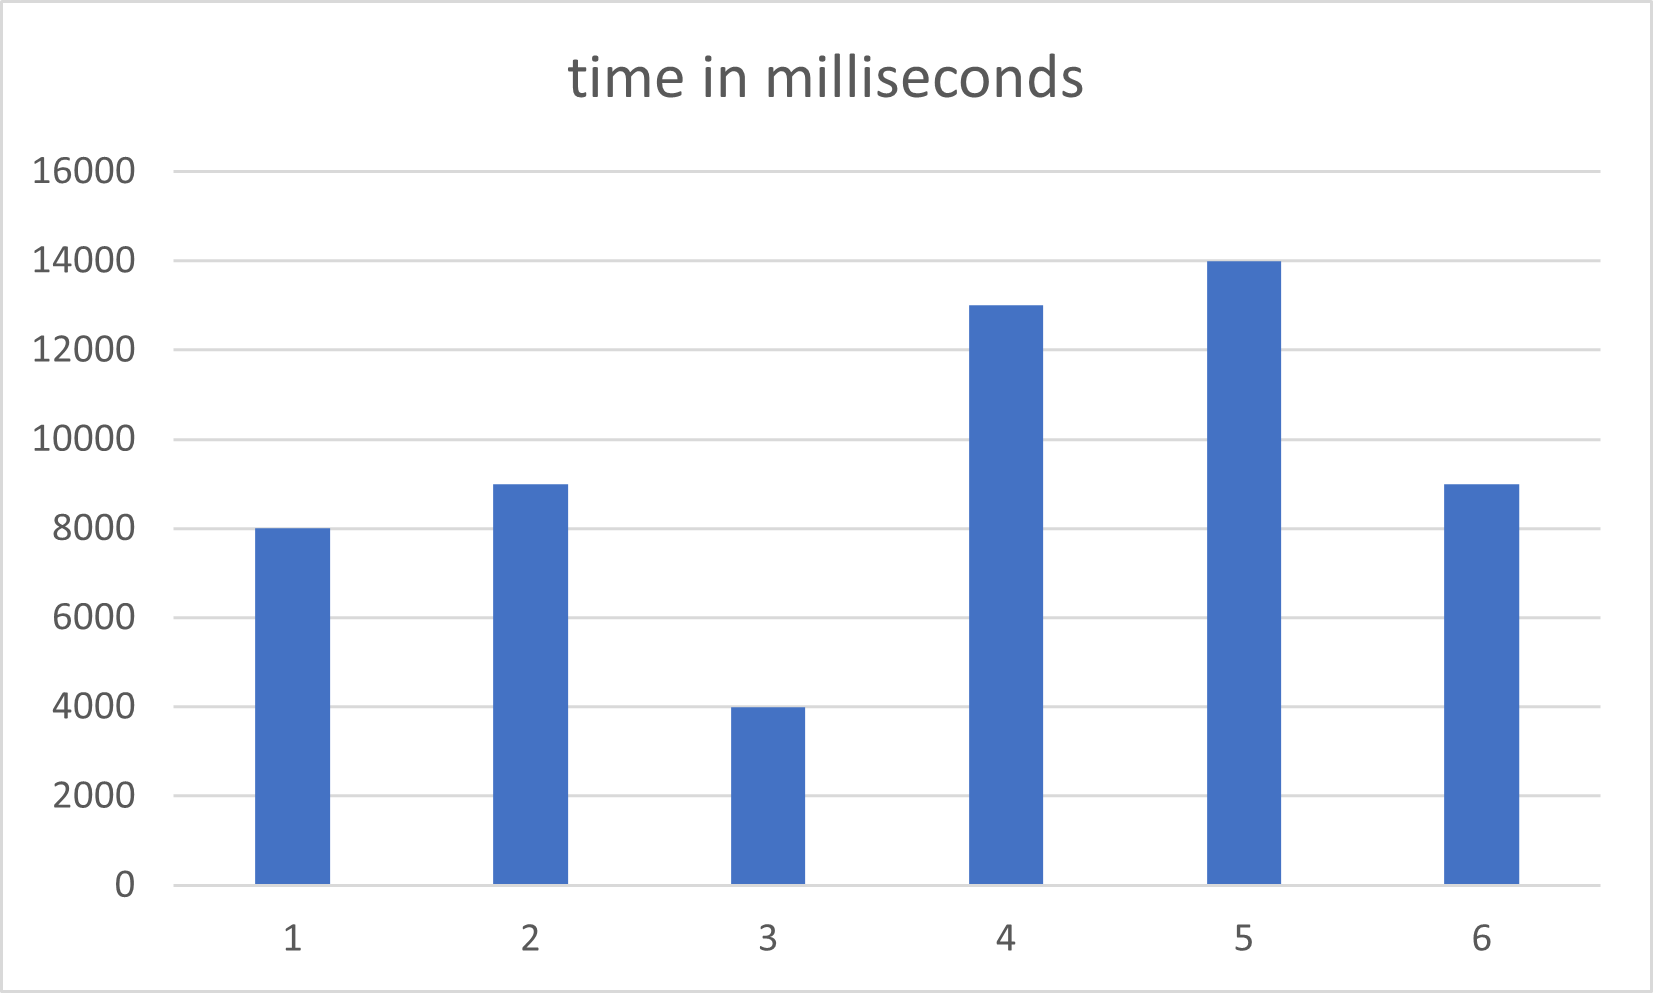
\includegraphics[width=0.99\textwidth, keepaspectratio]{content/07_evaluation_of_the_solution/ExcelPicture.png}
    \caption{Data loaded into excel}    
    \label{fig:Excel}
\end{figure}


\newpage\subsubsection*{T9: The experiment is redone a second time and another experimental setup is implemented}

The re-execution of an experiment verifying the requirement N5.1 can be implemented by re-reading the same experiment data. For this purpose, a generic experiment procedure was set up as an example, the experiment data was copied and used to perform a second experiment with the help of the artifact. At the same time, care was taken to ensure that the data of the participants in the two sample experiments were different. The second example experiment was congruent with the first experiment in terms of structure and execution. Only due to the different participant data, other attributes were queried in the questionair activity.

%just change the experiment data

    %\begin{lstlisting}[language=java,label=t3b,lineskip={0pt}, caption=Collect time needed to conduct experiment (b), basicstyle=\scriptsize, captionpos=b]
    %ArrayList<String> steps = new ArrayList<String>();

    %steps.add("com.example.master_thesis.InfoScreenActivity");
    %steps.add("com.example.master_thesis.ChooseTestSubjectActivity");
    %steps.add("com.example.master_thesis.QuestionnaireActivity");
    %steps.add("com.example.master_thesis.ChessExperimentActivity");
%\end{lstlisting}

\vspace{1cm}

\newpage\subsubsection*{T10: The experiment is conducted on different devices}

To verify requirement F5.2 and confirm test case T10, the developed artifact was exported to several other Android devices. Originally tested during development, the artifact was on a Pixel 4 XL. Therefore, to verify this test case, the artifact was installed and tested on a Pixel 6 Pro. The individual acitvities on this device are shown in Figure \ref{fig:uiScreensPixel6}. Although the two devices have different hardware, software and screen sizes, the artifact can be used on both devices and does not show any errors or bugs. This means that test case T10 can be fulfilled.

%PIXEL 6 PRO API 30
\vspace{1cm}

\begin{figure}[htbp]
    \centering
    \begin{subfigure}[b]{0.25\textwidth}
        \centering
        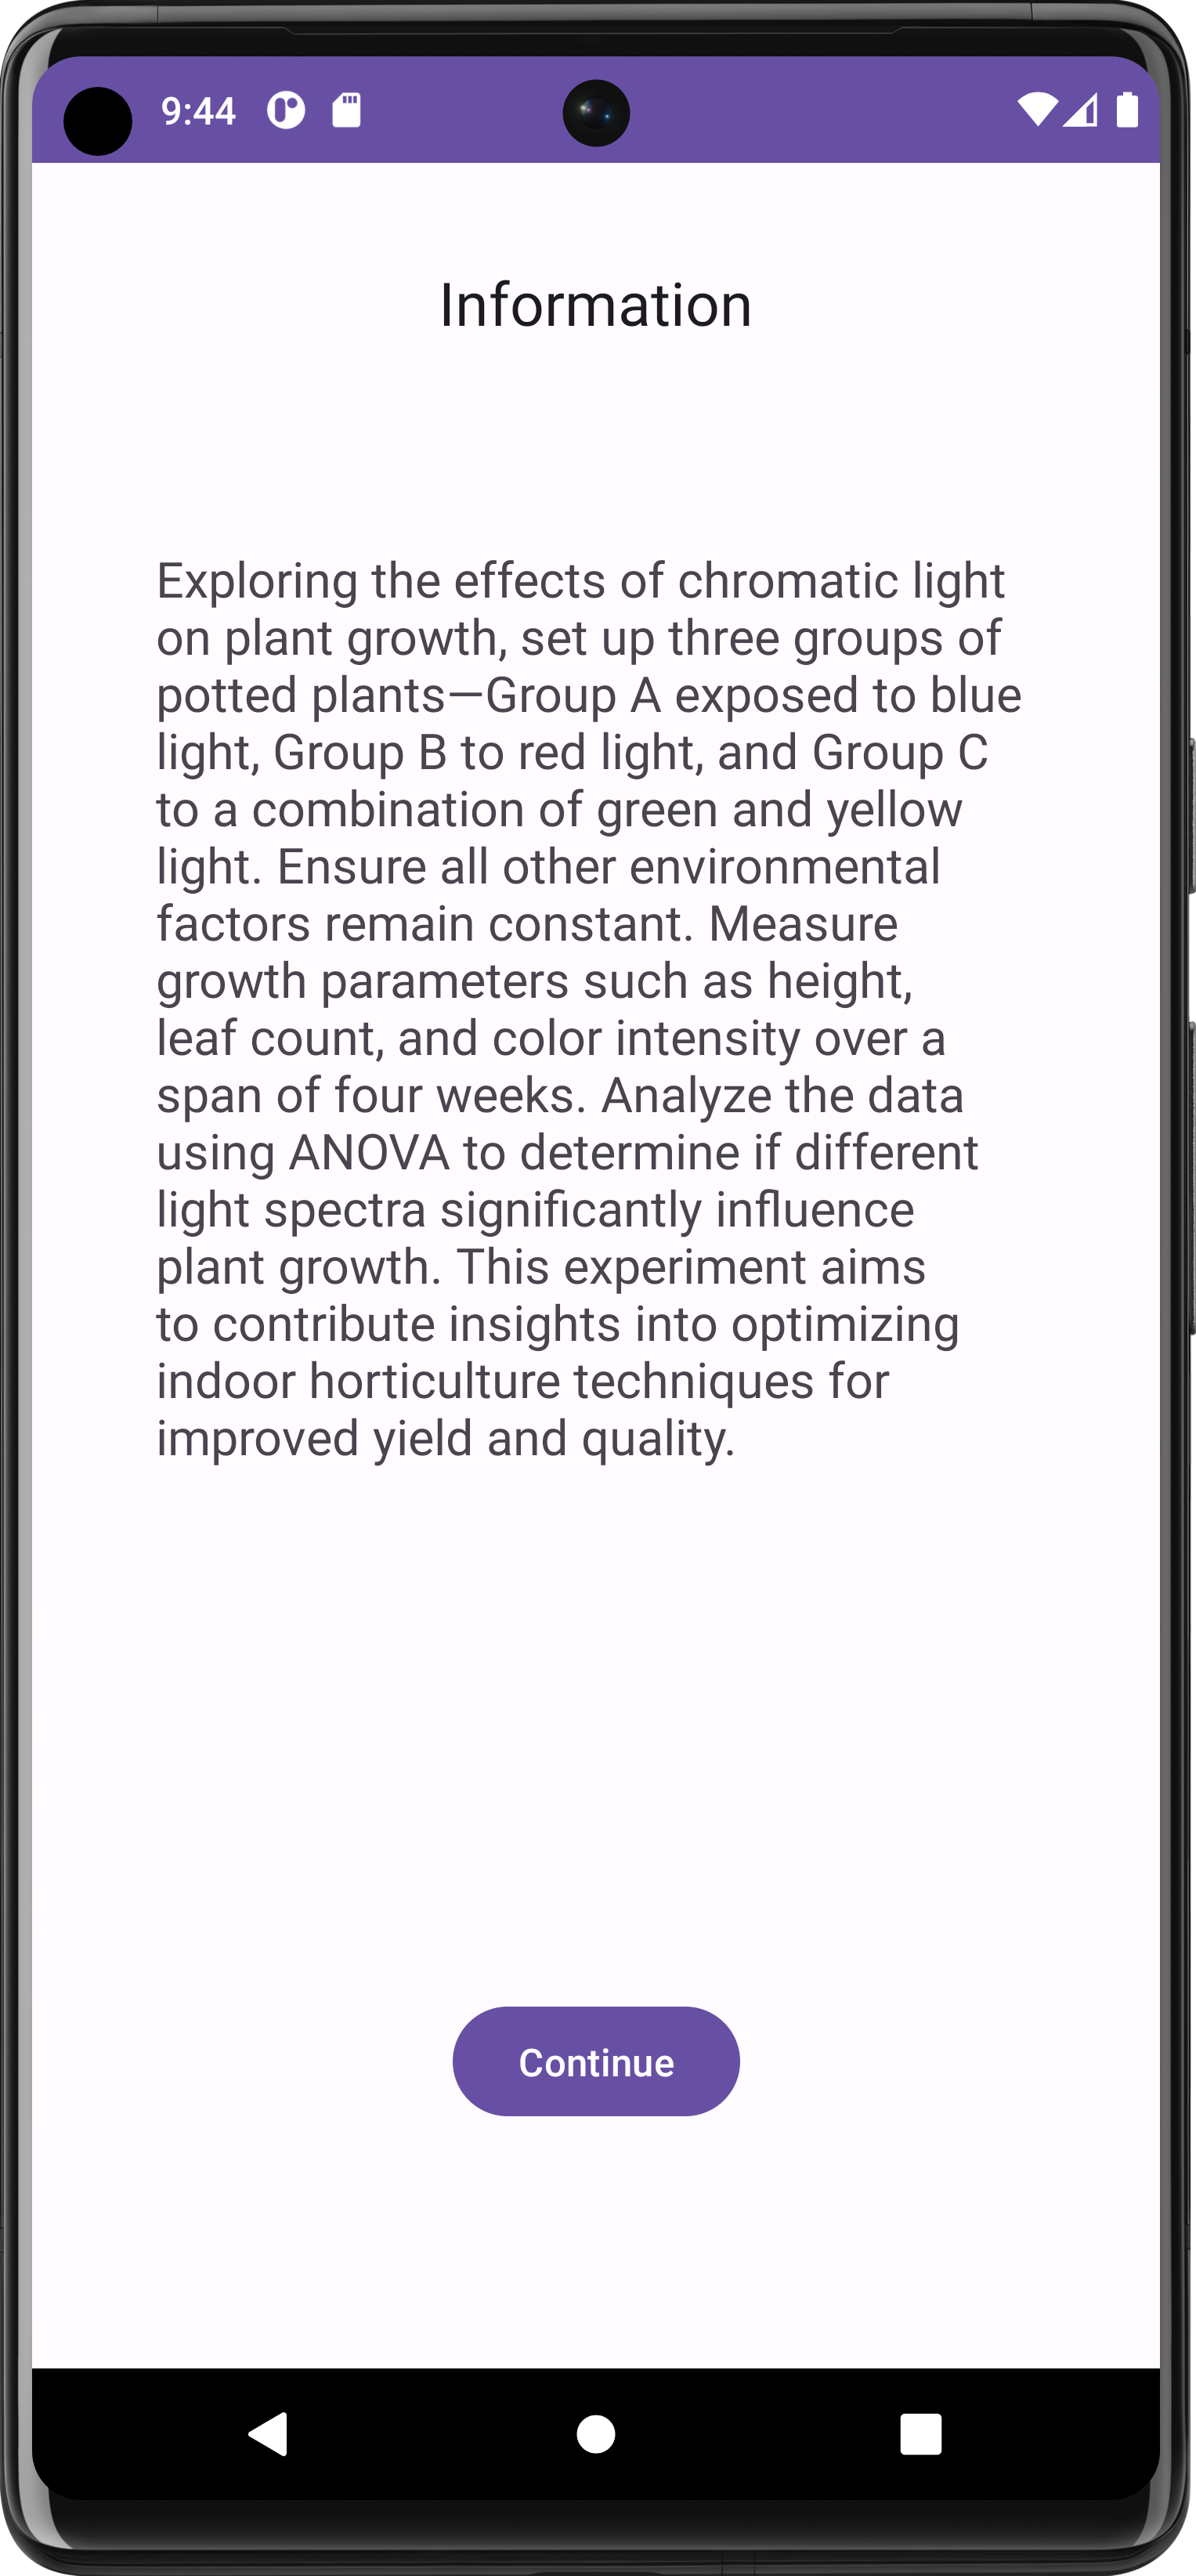
\includegraphics[width=\textwidth]{content/07_evaluation_of_the_solution/Screenshot_T10a.png}
        \caption{Info screen step | Pixel 6 Pro}
        \label{subfig:InfoScreenPixel}
    \end{subfigure}
        %\hfill
        \hspace{1cm}
    \begin{subfigure}[b]{0.25\textwidth}
        \centering
        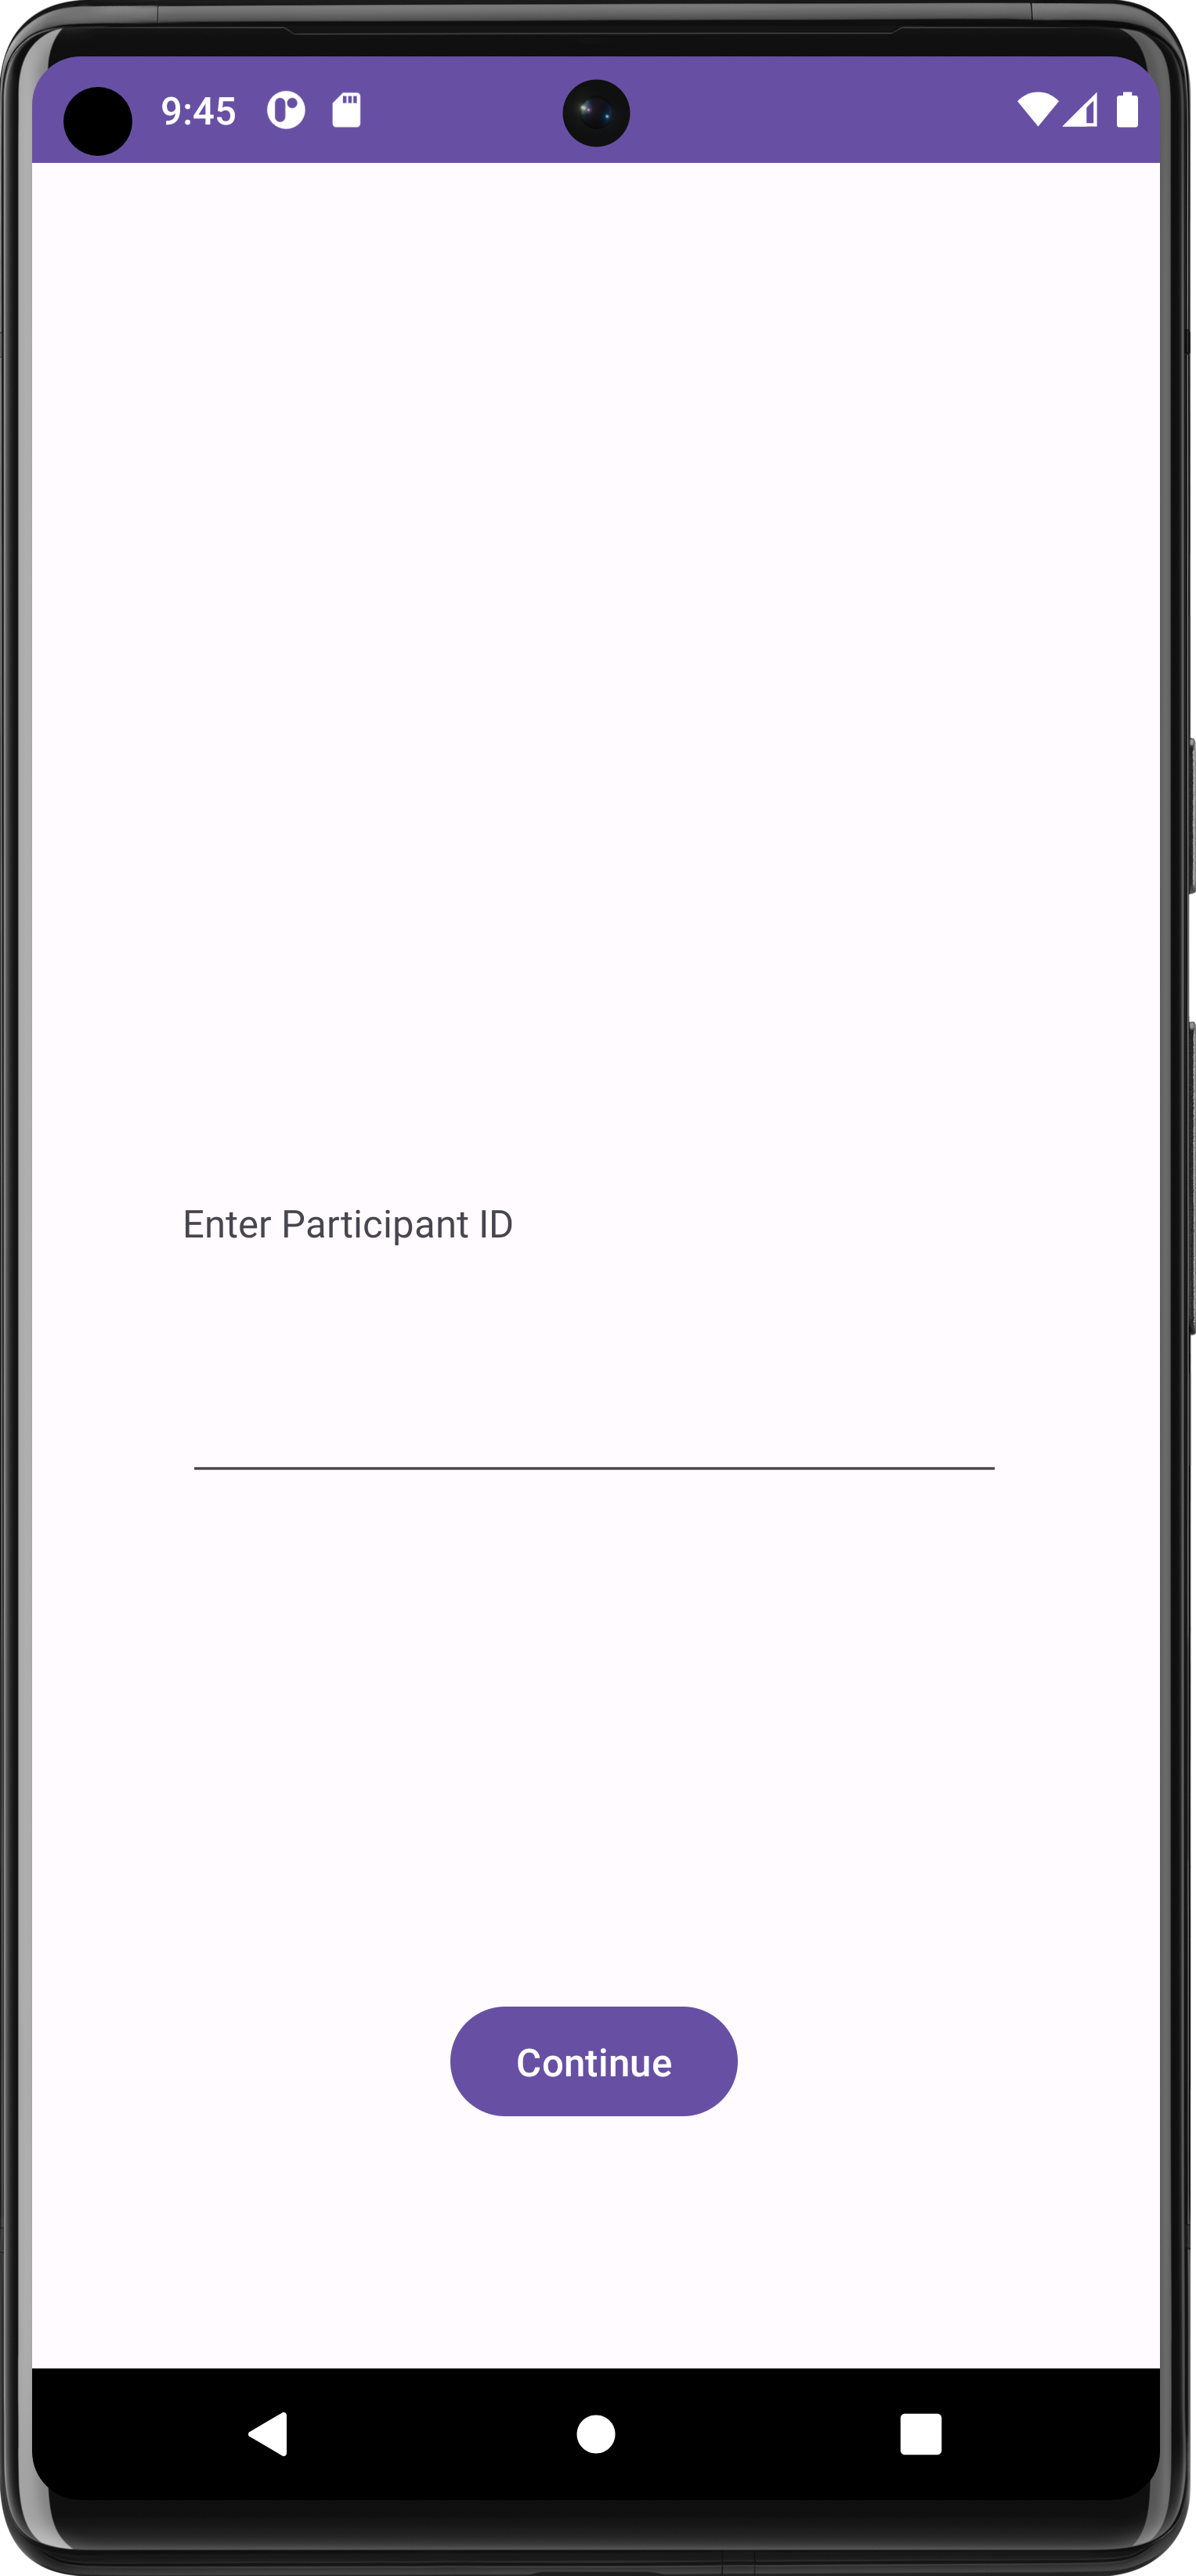
\includegraphics[width=\textwidth]{content/07_evaluation_of_the_solution/Screenshot_T10b.png}
        \caption{ Questionair step | Pixel 6 Pro}
        \label{subfig:QuestionairPixel}
    \end{subfigure}
        %\hfill
        \hspace{1cm}
    \begin{subfigure}[b]{0.25\textwidth}
        \centering
        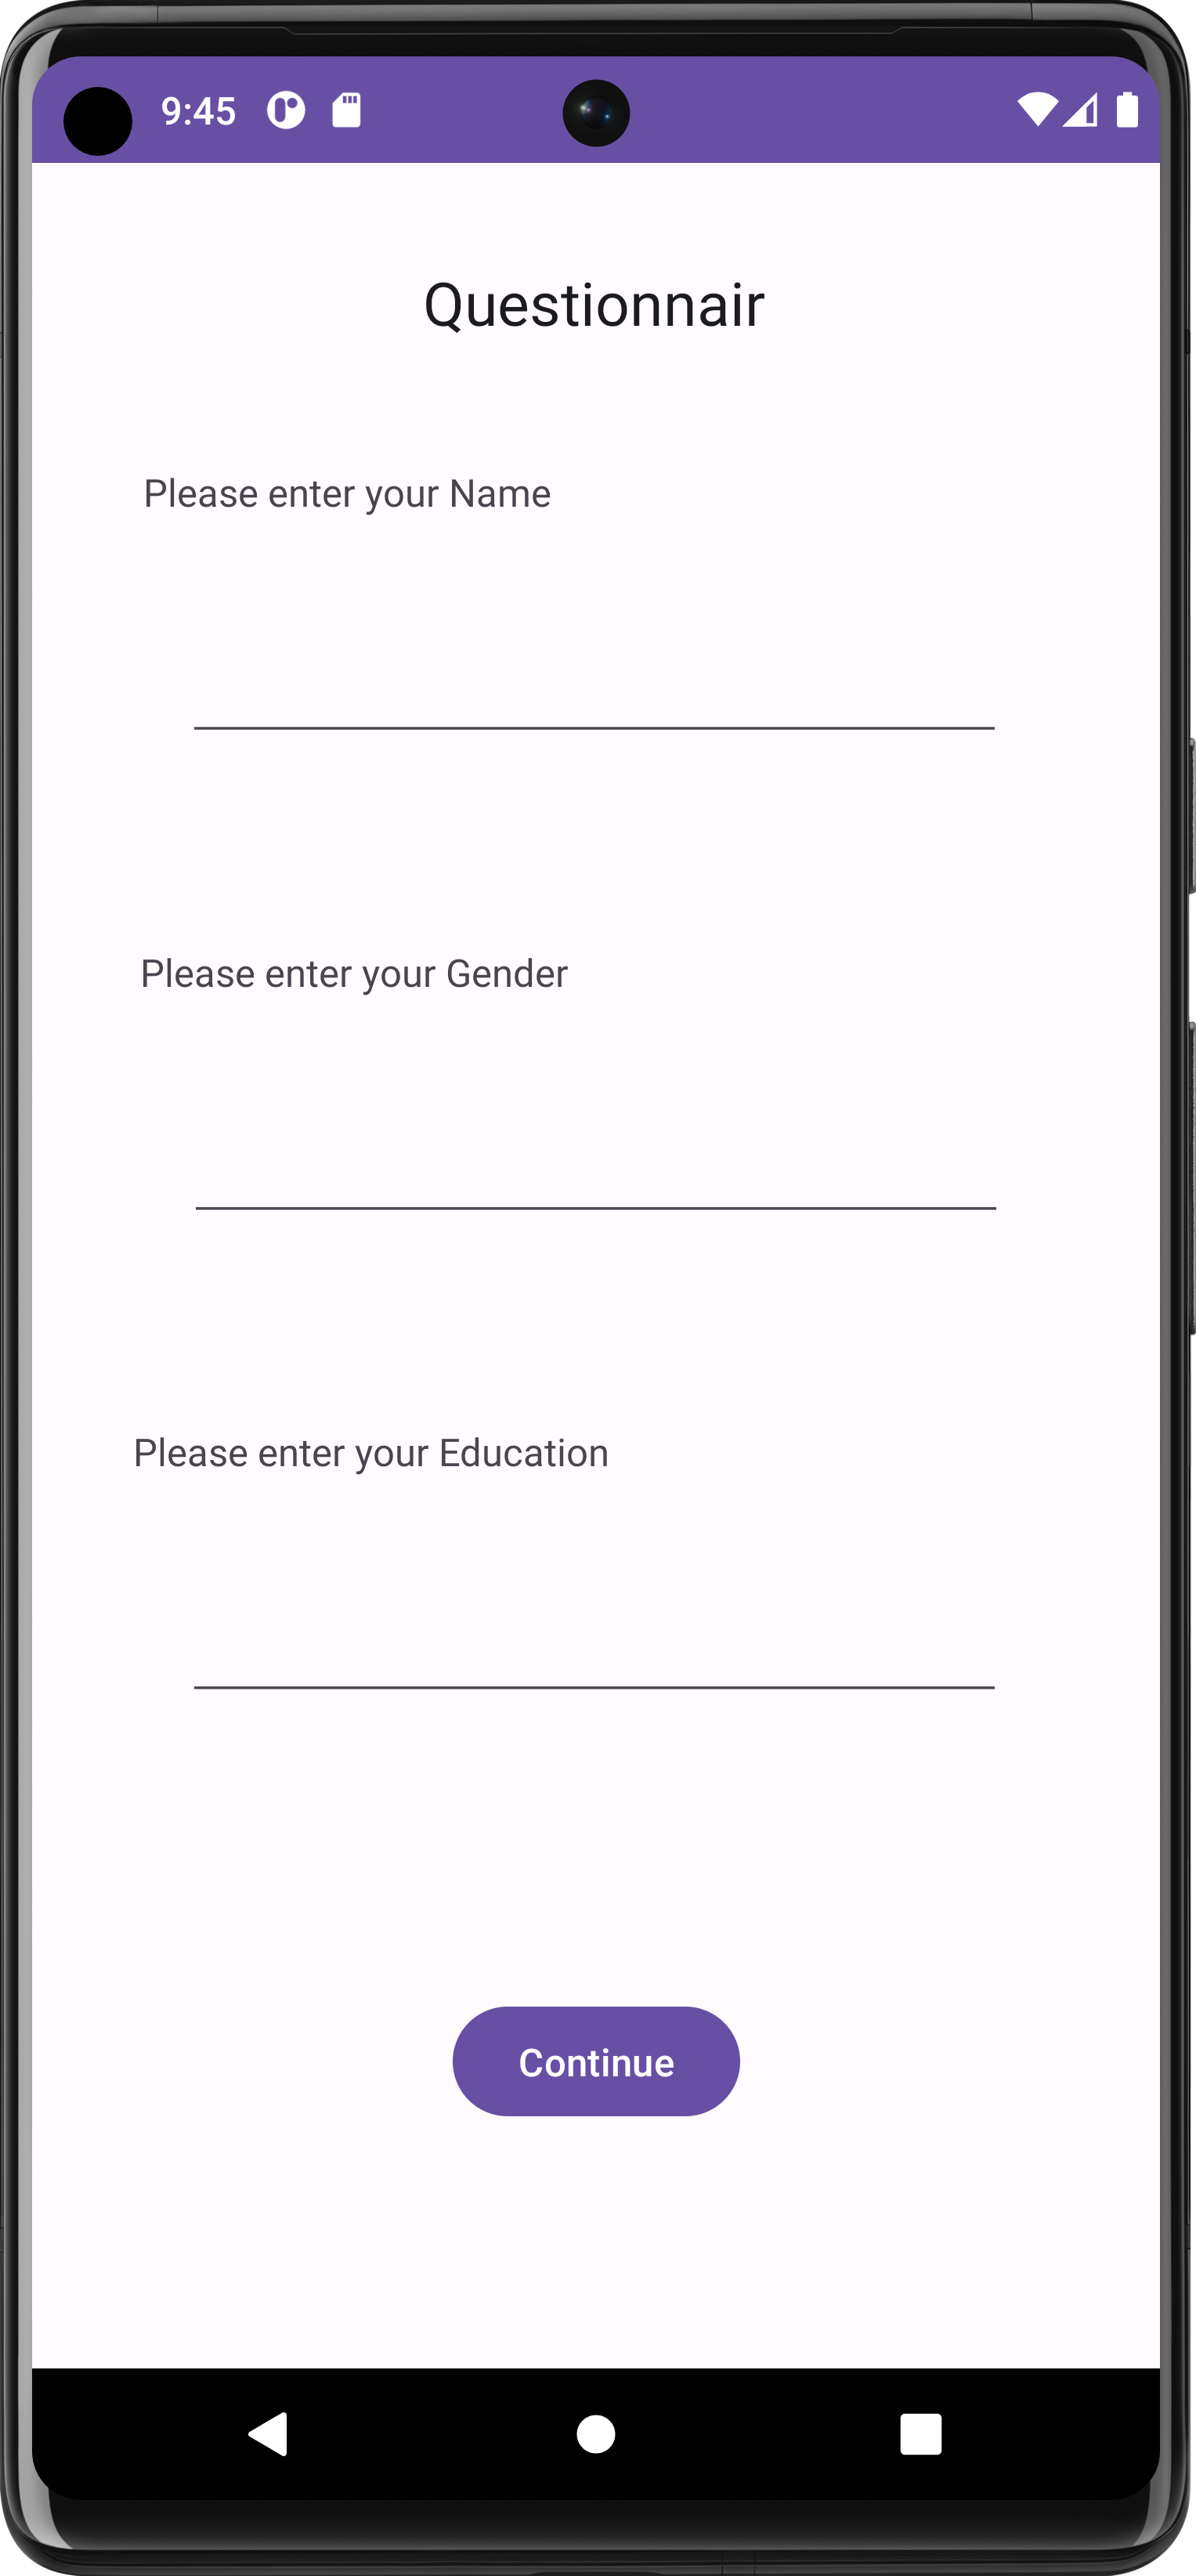
\includegraphics[width=\textwidth]{content/07_evaluation_of_the_solution/Screenshot_T10c.png}
        \caption{Choose test subject step | Pixel 6 Pro}
        \label{subfig:chooseTestSubjectPixel}
    \end{subfigure}
       \caption{Artefact run on a Pixel 6 Pro}
       \label{fig:uiScreensPixel6}
\end{figure}

\newpage\subsubsection*{T11: During the experiment the current state of the chess board is exported to the conducter of the experiment}

Test case T11 can be tested similarly to test case T7. For this purpose, a message about the current status of the experiment is sent to a server via a client class in the same way as in test case T7. In contrast to test case T7, no messages are sent back and forth, but only the current status of the experiment is exported to a monitor. Therefore, only one client class is needed in the application itself. The server to which the current status is sent can therefore take different forms, only the IP address of the server must be known and it must be able to process the client message. Analogous to test case T7, the implementation of this communication is also possible via other ways and means, should more complex functions be required that go beyond the capabilities of the Java sockets. Test case T11 and thus requirement N6.1 can thus be verified.


\subsubsection*{Remaining requirements}

In summary, all requirements could be verified with the help of the established test cases. One exception are the non-functional requirements N4.1 simplicity, N5.3 openness of platform and N8.1 advanced user interface, which cannot be verified by test cases due to their subjectivity. Nevertheless, as already discussed in section \ref{subsec:requirement_validation}, these requirements represent important specifications for the artifact. For this reason, the fulfillment of these non-functional requirements will be addressed as feasibly as possible without the use of test cases. For this purpose, the experience gained from the implementation of the artifact and the documentation on the individual technologies is used. Besides the fact that Android and Java are generally concidered to be simple beginner friendly technologies by the developer community, the best practice architecture that was implemented in the course of this application is a big indicator for the simplicity of the application. The individual functions and code modules have been divided into reusable UseCases and all user interface activities have been commulated into android activities. In addition, the implementation of new custom capabilities for individual experiments has been made extremely easy. For example, the definition of the experiment steps is realized through the experiment data and does not have to be implemented separately by program code. The implementation of custom experiments is also streamlined which makes it possible for the person performing the experiment to set up his experiment without having to worry about the basic framework. Despite the subjectivity of the "simplicity" requirement, the requirement N4.1 simplicity is considered to be fulfilled for the artefact due to the usage of technologies which are considered to be simple and beginner friendly, the reusable and streamlined best practice architecture and functionalities of the andoird application and the encapsulation of standard functionalities. 

Requirement

Requirement N5.3 Openness of platform describes the openness of the artifact for changes and enhancements. In general, it could be shown in the already verified requirements that the artifact is extensible. By using the best practice architecture in combination with the general concept of object orientation on which Java is based, it is also possible to argue that the application can be easily enhanced.





%\subsection{Prototype Testing}



\subsection{App Performance and Usability}
